\documentclass[12pt,a4paper]{article}

% Packages
\usepackage[utf8]{inputenc}
\usepackage[T1]{fontenc}
\usepackage{geometry}
\usepackage{graphicx}
\usepackage{xcolor}
\usepackage{colortbl}
\usepackage{amssymb}
\usepackage{listings}
\usepackage{hyperref}
\usepackage{booktabs}
\usepackage{longtable}
\usepackage{array}
\usepackage{tabularx}
\usepackage{fancyhdr}
\usepackage{titlesec}
\usepackage{enumitem}
\usepackage{tcolorbox}
\usepackage{tikz}
\usetikzlibrary{shapes.geometric, arrows, positioning, fit, calc}

% Page geometry
\geometry{
    left=2.5cm,
    right=2.5cm,
    top=3cm,
    bottom=3cm
}

% Colors
\definecolor{primaryblue}{RGB}{0, 82, 147}
\definecolor{secondaryblue}{RGB}{0, 120, 200}
\definecolor{lightgray}{RGB}{245, 245, 245}
\definecolor{darkgray}{RGB}{60, 60, 60}
\definecolor{successgreen}{RGB}{40, 167, 69}
\definecolor{warningorange}{RGB}{255, 193, 7}
\definecolor{errorred}{RGB}{220, 53, 69}
\definecolor{codebackground}{RGB}{248, 249, 250}

% Hyperref setup
\hypersetup{
    colorlinks=true,
    linkcolor=primaryblue,
    urlcolor=secondaryblue,
    citecolor=primaryblue
}

% Code listing style - removed language specifications
\lstdefinestyle{codestyle}{
    backgroundcolor=\color{codebackground},
    basicstyle=\ttfamily\small,
    breakatwhitespace=false,
    breaklines=true,
    captionpos=b,
    keepspaces=true,
    showspaces=false,
    showstringspaces=false,
    showtabs=false,
    tabsize=2,
    frame=single,
    rulecolor=\color{lightgray}
}
\lstset{style=codestyle}

% Header and footer
\pagestyle{fancy}
\fancyhf{}
\fancyhead[L]{\textcolor{primaryblue}{\textbf{OAuth 2.0 SSO Integration}}}
\fancyhead[R]{\textcolor{darkgray}{Technical Specification}}
\fancyfoot[C]{\thepage}
\renewcommand{\headrulewidth}{0.4pt}
\renewcommand{\footrulewidth}{0.4pt}

% Section formatting
\titleformat{\section}
    {\Large\bfseries\color{primaryblue}}
    {\thesection}{1em}{}[\titlerule]
\titleformat{\subsection}
    {\large\bfseries\color{secondaryblue}}
    {\thesubsection}{1em}{}
\titleformat{\subsubsection}
    {\normalsize\bfseries\color{darkgray}}
    {\thesubsubsection}{1em}{}

% Custom boxes
\tcbuselibrary{skins,breakable}

\newtcolorbox{infobox}[1][]{
    colback=blue!5,
    colframe=primaryblue,
    title=#1,
    fonttitle=\bfseries,
    breakable
}

\newtcolorbox{warningbox}[1][]{
    colback=orange!5,
    colframe=warningorange,
    title=#1,
    fonttitle=\bfseries,
    breakable
}

\newtcolorbox{successbox}[1][]{
    colback=green!5,
    colframe=successgreen,
    title=#1,
    fonttitle=\bfseries,
    breakable
}

\newtcolorbox{errorbox}[1][]{
    colback=red!5,
    colframe=errorred,
    title=#1,
    fonttitle=\bfseries,
    breakable
}

% Document info
\title{
    \vspace{-2cm}
    \textcolor{primaryblue}{\rule{\linewidth}{2pt}}\\[0.5cm]
    {\Huge\textbf{OAuth 2.0 Single Sign-On}}\\[0.3cm]
    {\LARGE\textbf{Integration Specification Document}}\\[0.5cm]
    \textcolor{primaryblue}{\rule{\linewidth}{2pt}}\\[1cm]
    {\Large Cross-Team Implementation Guide}\\[0.5cm]
    {\large App A (Java Authorization Server) $\longleftrightarrow$ App B (Next.js Client)}
}

\author{
    \textbf{Document Owner:} Team B (Next.js Application)\\
    \textbf{Version:} 1.0.0
}

\date{\textbf{Date:} January 3, 2026}

\begin{document}

\maketitle
\thispagestyle{empty}

\vfill

\begin{center}
\begin{tabular}{|l|l|}
\hline
\textbf{Document Status} & Draft / Under Review / Approved \\
\hline
\textbf{Classification} & Internal / Confidential \\
\hline
\textbf{Last Updated} & January 3, 2026 \\
\hline
\textbf{Review Date} & February 3, 2026 \\
\hline
\end{tabular}
\end{center}

\newpage

% Table of Contents
\tableofcontents
\newpage

%===============================================================================
% SECTION 1: EXECUTIVE SUMMARY
%===============================================================================
\section{Executive Summary}

\subsection{Purpose}
This document serves as the definitive technical specification for implementing OAuth 2.0 Single Sign-On (SSO) between two applications maintained by separate teams:

\begin{itemize}
    \item \textbf{App A (Authorization Server):} Java Web Application -- Maintained by Team A
    \item \textbf{App B (Client Application):} Next.js Application -- Maintained by Team B
\end{itemize}

\subsection{Scope}
This specification covers:
\begin{itemize}
    \item Complete OAuth 2.0 Authorization Code Flow with PKCE
    \item All API endpoints required from both teams
    \item Frontend URLs and routes
    \item Data exchange formats and contracts
    \item Security requirements
    \item Integration testing procedures
\end{itemize}

\subsection{Audience}
\begin{itemize}
    \item Backend Developers (Team A and Team B)
    \item Frontend Developers (Team A and Team B)
    \item DevOps Engineers
    \item Security Architects
    \item Project Managers
\end{itemize}

%===============================================================================
% SECTION 2: SYSTEM OVERVIEW
%===============================================================================
\newpage
\section{System Overview}

\subsection{Architecture Diagram}

\begin{center}
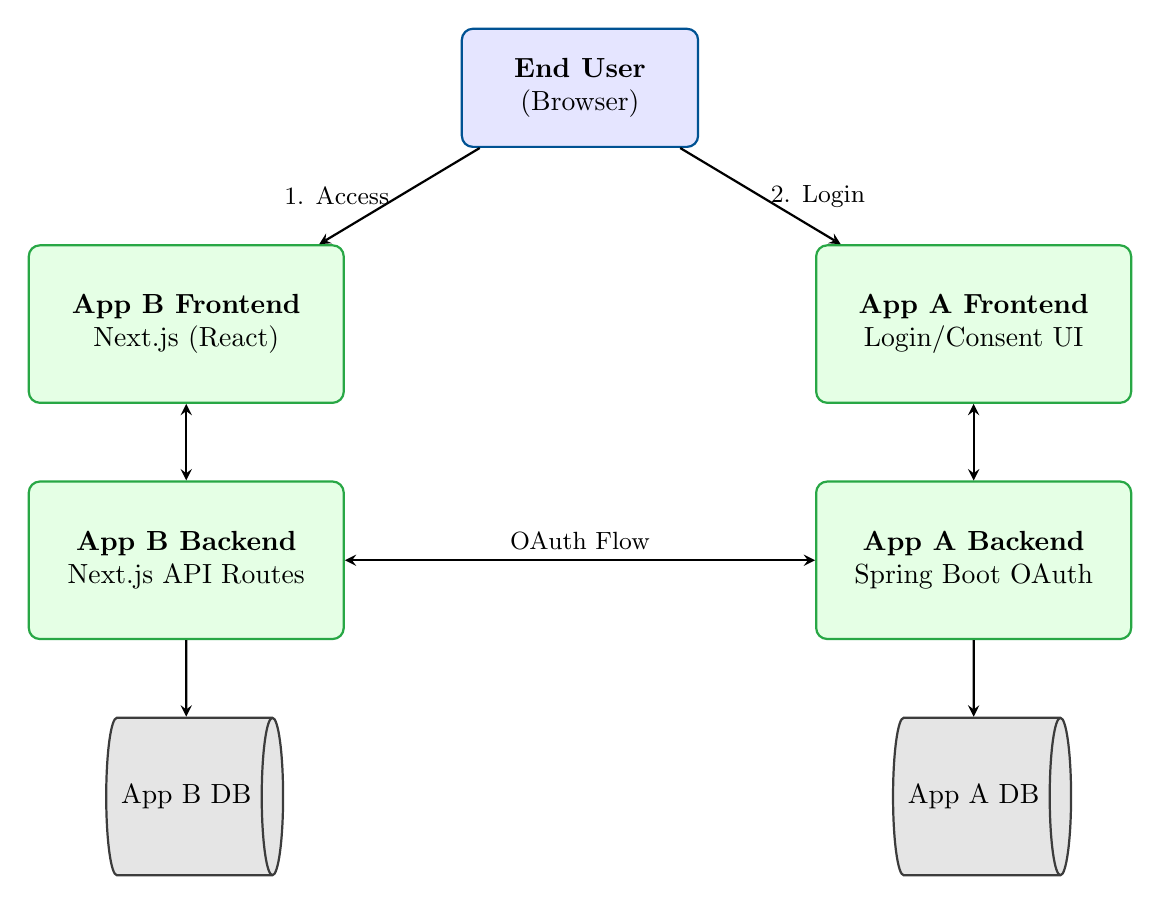
\begin{tikzpicture}[
    node distance=2cm,
    box/.style={rectangle, draw=primaryblue, fill=blue!10, thick, minimum width=3cm, minimum height=1.5cm, text centered, rounded corners, align=center},
    serverbox/.style={rectangle, draw=successgreen, fill=green!10, thick, minimum width=4cm, minimum height=2cm, text centered, rounded corners, align=center},
    dbbox/.style={cylinder, draw=darkgray, fill=gray!20, thick, minimum width=2cm, minimum height=1.5cm, text centered, aspect=0.5, align=center},
    arrow/.style={->, thick, >=stealth}
]

% User
\node[box] (user) at (0,0) {\textbf{End User}\\(Browser)};

% App B
\node[serverbox] (appb-frontend) at (-5,-3) {\textbf{App B Frontend}\\Next.js (React)};
\node[serverbox] (appb-backend) at (-5,-6) {\textbf{App B Backend}\\Next.js API Routes};

% App A
\node[serverbox] (appa-frontend) at (5,-3) {\textbf{App A Frontend}\\Login/Consent UI};
\node[serverbox] (appa-backend) at (5,-6) {\textbf{App A Backend}\\Spring Boot OAuth};

% Databases
\node[dbbox] (appb-db) at (-5,-9) {App B DB};
\node[dbbox] (appa-db) at (5,-9) {App A DB};

% Arrows
\draw[arrow] (user) -- node[left, font=\small] {1. Access} (appb-frontend);
\draw[arrow] (user) -- node[right, font=\small] {2. Login} (appa-frontend);
\draw[arrow, <->] (appb-frontend) -- (appb-backend);
\draw[arrow, <->] (appa-frontend) -- (appa-backend);
\draw[arrow, <->] (appb-backend) -- node[above, font=\small] {OAuth Flow} (appa-backend);
\draw[arrow] (appb-backend) -- (appb-db);
\draw[arrow] (appa-backend) -- (appa-db);

\end{tikzpicture}
\end{center}

\subsection{OAuth 2.0 Flow Sequence}

\begin{center}
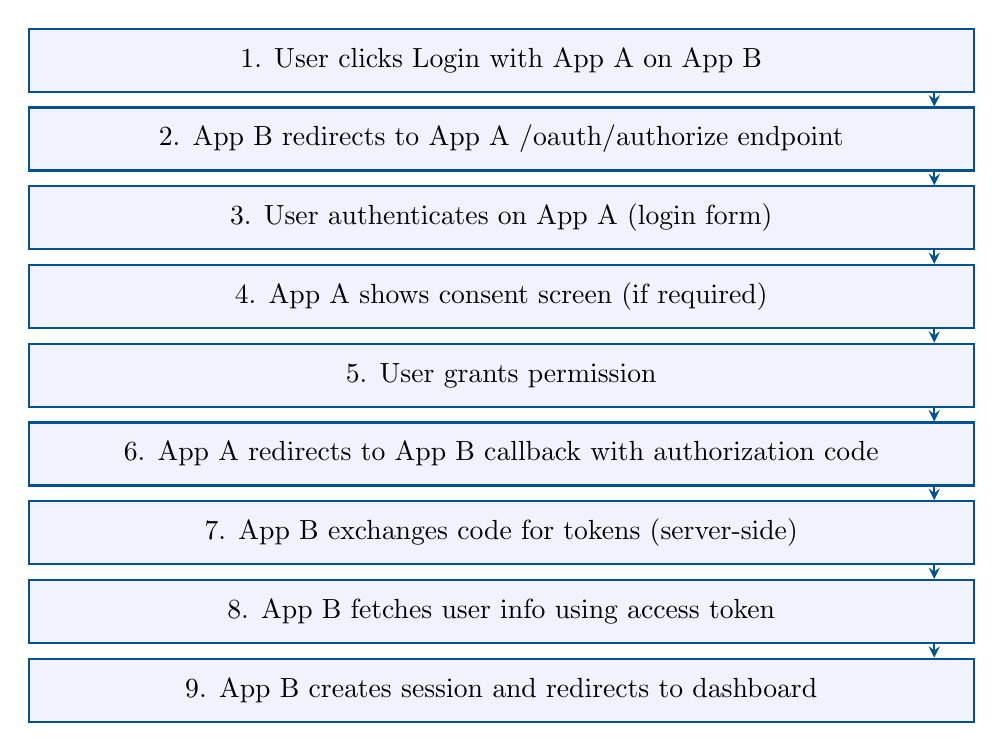
\begin{tikzpicture}[
    node distance=0.5cm,
    stepbox/.style={rectangle, draw=primaryblue, fill=blue!5, thick, minimum width=12cm, minimum height=0.8cm, text centered, align=center},
    arrow/.style={->, thick, >=stealth, primaryblue}
]

\node[stepbox] (s1) at (0,0) {1. User clicks Login with App A on App B};
\node[stepbox] (s2) at (0,-1) {2. App B redirects to App A /oauth/authorize endpoint};
\node[stepbox] (s3) at (0,-2) {3. User authenticates on App A (login form)};
\node[stepbox] (s4) at (0,-3) {4. App A shows consent screen (if required)};
\node[stepbox] (s5) at (0,-4) {5. User grants permission};
\node[stepbox] (s6) at (0,-5) {6. App A redirects to App B callback with authorization code};
\node[stepbox] (s7) at (0,-6) {7. App B exchanges code for tokens (server-side)};
\node[stepbox] (s8) at (0,-7) {8. App B fetches user info using access token};
\node[stepbox] (s9) at (0,-8) {9. App B creates session and redirects to dashboard};

\foreach \i in {1,...,8} {
    \pgfmathtruncatemacro{\j}{\i+1}
    \draw[arrow] ([xshift=5.5cm]s\i.south) -- ([xshift=5.5cm]s\j.north);
}

\end{tikzpicture}
\end{center}

%===============================================================================
% SECTION 3: WHAT TEAM B PROVIDES TO TEAM A
%===============================================================================
\newpage
\section{What Team B (Next.js) Provides to Team A}

\begin{infobox}[Team B Deliverables]
This section details all information, URLs, and configurations that Team B must provide to Team A for OAuth client registration.
\end{infobox}

\subsection{Application Registration Information}

\begin{center}
\begin{tabular}{|p{4cm}|p{5cm}|p{5cm}|}
\hline
\rowcolor{primaryblue!20}
\textbf{Field} & \textbf{Description} & \textbf{Example Value} \\
\hline
Application Name & Display name shown on consent screen & My Next.js Application \\
\hline
Application Description & Brief description of what App B does & A modern web application \\
\hline
Application Logo URL & Logo to display on consent screen & https://app-b.com/logo.png \\
\hline
Application Website & Main website URL & https://app-b.com \\
\hline
Privacy Policy URL & Link to privacy policy & https://app-b.com/privacy \\
\hline
Terms of Service URL & Link to terms of service & https://app-b.com/terms \\
\hline
Technical Contact & For technical issues & dev@app-b.com \\
\hline
Support Contact & For user support & support@app-b.com \\
\hline
\end{tabular}
\end{center}

\subsection{Redirect URIs (Callback URLs)}

\begin{warningbox}[Critical: Exact Match Required]
Redirect URIs must match EXACTLY. Pay attention to:
\begin{itemize}
    \item Protocol (http vs https)
    \item Trailing slashes
    \item Port numbers
    \item Case sensitivity
\end{itemize}
\end{warningbox}

\subsubsection{Production Environment}
\begin{lstlisting}
https://app-b.example.com/auth/callback
https://app-b.example.com/api/auth/callback
\end{lstlisting}

\subsubsection{Staging Environment}
\begin{lstlisting}
https://staging.app-b.example.com/auth/callback
https://staging.app-b.example.com/api/auth/callback
\end{lstlisting}

\subsubsection{Development Environment}
\begin{lstlisting}
http://localhost:3000/auth/callback
http://localhost:3000/api/auth/callback
http://127.0.0.1:3000/auth/callback
\end{lstlisting}

\subsection{Post-Logout Redirect URIs}

\begin{lstlisting}
Production:
https://app-b.example.com
https://app-b.example.com/auth/login

Staging:
https://staging.app-b.example.com
https://staging.app-b.example.com/auth/login

Development:
http://localhost:3000
http://localhost:3000/auth/login
\end{lstlisting}

\subsection{Required OAuth Scopes}

\begin{center}
\begin{tabular}{|l|l|p{6cm}|}
\hline
\rowcolor{primaryblue!20}
\textbf{Scope} & \textbf{Required} & \textbf{Purpose} \\
\hline
openid & Yes & Enable OpenID Connect authentication \\
\hline
profile & Yes & Access user name, picture \\
\hline
email & Yes & Access user email address \\
\hline
offline\_access & Optional & Enable refresh tokens \\
\hline
\end{tabular}
\end{center}

\subsection{Technical Requirements}

\begin{center}
\begin{tabular}{|p{5cm}|p{9cm}|}
\hline
\rowcolor{primaryblue!20}
\textbf{Requirement} & \textbf{Value/Details} \\
\hline
PKCE Support & Required (code\_challenge\_method: S256) \\
\hline
Token Storage & Server-side only (HTTP-only cookies) \\
\hline
State Parameter & Will be used (cryptographically random) \\
\hline
Grant Types Needed & authorization\_code, refresh\_token \\
\hline
Response Type & code \\
\hline
\end{tabular}
\end{center}

%===============================================================================
% SECTION 4: WHAT TEAM A PROVIDES TO TEAM B
%===============================================================================
\newpage
\section{What Team A (Java) Provides to Team B}

\begin{infobox}[Team A Deliverables]
This section details all credentials, endpoints, and configurations that Team A must provide to Team B after client registration.
\end{infobox}

\subsection{OAuth Client Credentials}

\begin{center}
\begin{tabular}{|p{4cm}|p{5cm}|p{5cm}|}
\hline
\rowcolor{successgreen!20}
\textbf{Credential} & \textbf{Description} & \textbf{Example Format} \\
\hline
Client ID & Public identifier for App B & app-b-prod-abc123xyz \\
\hline
Client Secret & Secret key for token exchange & sk\_live\_AbCdEf123456... \\
\hline
\end{tabular}
\end{center}

\begin{errorbox}[Security Warning]
\textbf{Client Secret Handling:}
\begin{itemize}
    \item NEVER commit to version control
    \item NEVER expose in frontend/client-side code
    \item Store in environment variables or secret manager
    \item Transmit via secure channel (encrypted email, secret manager)
\end{itemize}
\end{errorbox}

\subsection{Authorization Server Base URLs}

\begin{center}
\begin{tabular}{|l|l|}
\hline
\rowcolor{successgreen!20}
\textbf{Environment} & \textbf{Base URL} \\
\hline
Production & https://auth.example.com \\
\hline
Staging & https://auth-staging.example.com \\
\hline
Development & http://localhost:4000 \\
\hline
\end{tabular}
\end{center}

\subsection{OAuth Endpoints (Team A Must Implement)}

\subsubsection{Authorization Endpoint}

\begin{successbox}[GET /oauth/authorize]
\textbf{Full URL:} \texttt{https://auth.example.com/oauth/authorize}

\textbf{Purpose:} Initiates OAuth flow, displays login/consent UI

\textbf{Query Parameters:}
\begin{center}
\begin{tabular}{|l|l|l|p{4.5cm}|}
\hline
\rowcolor{gray!20}
\textbf{Parameter} & \textbf{Required} & \textbf{Type} & \textbf{Description} \\
\hline
client\_id & Yes & string & App B client ID \\
\hline
redirect\_uri & Yes & string & Callback URL (registered) \\
\hline
response\_type & Yes & string & Must be code \\
\hline
scope & Yes & string & Space-separated scopes \\
\hline
state & Yes & string & Random CSRF token \\
\hline
code\_challenge & Yes & string & PKCE challenge (base64url) \\
\hline
code\_challenge\_method & Yes & string & Must be S256 \\
\hline
\end{tabular}
\end{center}

\textbf{Success Response:} Redirects to redirect\_uri with:
\begin{lstlisting}
https://app-b.com/auth/callback?code=AUTH_CODE&state=STATE_VALUE
\end{lstlisting}

\textbf{Error Response:} Redirects to redirect\_uri with:
\begin{lstlisting}
https://app-b.com/auth/callback?error=ERROR_CODE&error_description=DESC&state=STATE
\end{lstlisting}
\end{successbox}

\subsubsection{Token Endpoint}

\begin{successbox}[POST /oauth/token]
\textbf{Full URL:} \texttt{https://auth.example.com/oauth/token}

\textbf{Purpose:} Exchange authorization code for tokens / Refresh tokens

\textbf{Headers:}
\begin{lstlisting}
Content-Type: application/x-www-form-urlencoded
\end{lstlisting}

\textbf{Request Body (Authorization Code Grant):}
\begin{lstlisting}
grant_type=authorization_code
&code=AUTHORIZATION_CODE
&redirect_uri=https://app-b.com/auth/callback
&client_id=CLIENT_ID
&client_secret=CLIENT_SECRET
&code_verifier=CODE_VERIFIER
\end{lstlisting}

\textbf{Request Body (Refresh Token Grant):}
\begin{lstlisting}
grant_type=refresh_token
&refresh_token=REFRESH_TOKEN
&client_id=CLIENT_ID
&client_secret=CLIENT_SECRET
\end{lstlisting}

\textbf{Success Response (200 OK):}
\begin{lstlisting}
{
    "access_token": "eyJhbGciOiJSUzI1NiIsInR5cCI6IkpXVCJ9...",
    "token_type": "Bearer",
    "expires_in": 3600,
    "refresh_token": "dGhpcyBpcyBhIHJlZnJlc2ggdG9rZW4...",
    "scope": "openid profile email",
    "id_token": "eyJhbGciOiJSUzI1NiIsInR5cCI6IkpXVCJ9..."
}
\end{lstlisting}

\textbf{Error Response (400 Bad Request):}
\begin{lstlisting}
{
    "error": "invalid_grant",
    "error_description": "The authorization code has expired"
}
\end{lstlisting}
\end{successbox}

\subsubsection{UserInfo Endpoint}

\begin{successbox}[GET /oauth/userinfo]
\textbf{Full URL:} \texttt{https://auth.example.com/oauth/userinfo}

\textbf{Purpose:} Retrieve authenticated user profile

\textbf{Headers:}
\begin{lstlisting}
Authorization: Bearer ACCESS_TOKEN
\end{lstlisting}

\textbf{Success Response (200 OK):}
\begin{lstlisting}
{
    "sub": "user-uuid-12345",
    "email": "user@example.com",
    "email_verified": true,
    "name": "John Doe",
    "given_name": "John",
    "family_name": "Doe",
    "picture": "https://example.com/avatar.jpg",
    "updated_at": 1609459200
}
\end{lstlisting}

\textbf{Error Response (401 Unauthorized):}
\begin{lstlisting}
{
    "error": "invalid_token",
    "error_description": "The access token is expired"
}
\end{lstlisting}
\end{successbox}

\subsubsection{Token Revocation Endpoint}

\begin{successbox}[POST /oauth/revoke]
\textbf{Full URL:} \texttt{https://auth.example.com/oauth/revoke}

\textbf{Purpose:} Revoke access or refresh tokens

\textbf{Headers:}
\begin{lstlisting}
Content-Type: application/x-www-form-urlencoded
\end{lstlisting}

\textbf{Request Body:}
\begin{lstlisting}
token=TOKEN_TO_REVOKE
&token_type_hint=refresh_token
&client_id=CLIENT_ID
&client_secret=CLIENT_SECRET
\end{lstlisting}

\textbf{Response:} HTTP 200 OK (always, even if token invalid)
\end{successbox}

\subsubsection{JWKS Endpoint}

\begin{successbox}[GET /.well-known/jwks.json]
\textbf{Full URL:} \texttt{https://auth.example.com/.well-known/jwks.json}

\textbf{Purpose:} Public keys for JWT verification

\textbf{Response:}
\begin{lstlisting}
{
    "keys": [
        {
            "kty": "RSA",
            "kid": "key-id-1",
            "use": "sig",
            "alg": "RS256",
            "n": "base64url-encoded-modulus...",
            "e": "AQAB"
        }
    ]
}
\end{lstlisting}
\end{successbox}

\subsubsection{OpenID Configuration Endpoint}

\begin{successbox}[GET /.well-known/openid-configuration]
\textbf{Full URL:} \texttt{https://auth.example.com/.well-known/openid-configuration}

\textbf{Purpose:} OAuth/OIDC discovery document

\textbf{Response:}
\begin{lstlisting}
{
    "issuer": "https://auth.example.com",
    "authorization_endpoint": "https://auth.example.com/oauth/authorize",
    "token_endpoint": "https://auth.example.com/oauth/token",
    "userinfo_endpoint": "https://auth.example.com/oauth/userinfo",
    "revocation_endpoint": "https://auth.example.com/oauth/revoke",
    "jwks_uri": "https://auth.example.com/.well-known/jwks.json",
    "response_types_supported": ["code"],
    "grant_types_supported": ["authorization_code", "refresh_token"],
    "scopes_supported": ["openid", "profile", "email"],
    "token_endpoint_auth_methods_supported": ["client_secret_post"],
    "code_challenge_methods_supported": ["S256"]
}
\end{lstlisting}
\end{successbox}

\subsection{Token Configuration}

\begin{center}
\begin{tabular}{|p{5cm}|p{4cm}|p{5cm}|}
\hline
\rowcolor{successgreen!20}
\textbf{Configuration} & \textbf{Value} & \textbf{Notes} \\
\hline
Access Token Lifetime & 3600 seconds (1 hour) & Refresh before expiry \\
\hline
Refresh Token Lifetime & 604800 seconds (7 days) & Rotate on use \\
\hline
Authorization Code Lifetime & 600 seconds (10 min) & Single use only \\
\hline
ID Token Algorithm & RS256 & Asymmetric signing \\
\hline
Token Type & Bearer & Standard bearer token \\
\hline
\end{tabular}
\end{center}

\subsection{Frontend Pages (Team A Must Implement)}

\begin{center}
\begin{tabular}{|p{4cm}|p{4cm}|p{6cm}|}
\hline
\rowcolor{successgreen!20}
\textbf{Page} & \textbf{URL} & \textbf{Description} \\
\hline
Login Page & /login & User authentication form \\
\hline
Registration Page & /register & New user registration \\
\hline
Consent Screen & /oauth/consent & Permission approval screen \\
\hline
Password Reset & /forgot-password & Password recovery flow \\
\hline
Error Page & /oauth/error & OAuth error display \\
\hline
\end{tabular}
\end{center}

%===============================================================================
% SECTION 5: WHAT TEAM B MUST IMPLEMENT
%===============================================================================
\newpage
\section{What Team B (Next.js) Must Implement}

\begin{infobox}[Team B Implementation Requirements]
This section details all endpoints, pages, and components that Team B must build.
\end{infobox}

\subsection{Backend API Routes}

\subsubsection{Login Initiation Route}

\begin{successbox}[GET /api/auth/login]
\textbf{Purpose:} Generate OAuth URL and redirect to App A

\textbf{Implementation Steps:}
\begin{enumerate}
    \item Generate cryptographically random \texttt{state} value
    \item Generate PKCE \texttt{code\_verifier} (43-128 characters)
    \item Calculate \texttt{code\_challenge} = base64url(SHA256(code\_verifier))
    \item Store state and code\_verifier in HTTP-only cookies
    \item Build authorization URL with all parameters
    \item Redirect user to App A authorization endpoint
\end{enumerate}

\textbf{Response:} HTTP 302 Redirect to App A
\end{successbox}

\subsubsection{OAuth Callback Route}

\begin{successbox}[GET /api/auth/callback]
\textbf{Purpose:} Handle callback from App A, exchange code for tokens

\textbf{Query Parameters Received:}
\begin{itemize}
    \item \texttt{code} - Authorization code (on success)
    \item \texttt{state} - State parameter for validation
    \item \texttt{error} - Error code (on failure)
    \item \texttt{error\_description} - Error details (on failure)
\end{itemize}

\textbf{Implementation Steps:}
\begin{enumerate}
    \item Validate \texttt{state} matches stored value
    \item Check for \texttt{error} parameter
    \item Retrieve stored \texttt{code\_verifier}
    \item Call App A token endpoint with code
    \item Call App A userinfo endpoint
    \item Create session with tokens and user info
    \item Clear OAuth cookies
    \item Redirect to dashboard
\end{enumerate}

\textbf{Response:} HTTP 302 Redirect to /dashboard or /auth/login?error=...
\end{successbox}

\subsubsection{Token Refresh Route}

\begin{successbox}[POST /api/auth/refresh]
\textbf{Purpose:} Refresh expired access token

\textbf{Implementation Steps:}
\begin{enumerate}
    \item Get session from request
    \item Extract refresh token
    \item Call App A token endpoint with refresh\_token grant
    \item Update session with new tokens
    \item Return success/failure
\end{enumerate}

\textbf{Success Response:}
\begin{lstlisting}
{
    "success": true
}
\end{lstlisting}

\textbf{Error Response:}
\begin{lstlisting}
{
    "error": "refresh_failed",
    "message": "Please login again"
}
\end{lstlisting}
\end{successbox}

\subsubsection{Logout Route}

\begin{successbox}[POST /api/auth/logout]
\textbf{Purpose:} Revoke tokens and clear session

\textbf{Implementation Steps:}
\begin{enumerate}
    \item Get session from request
    \item Call App A revoke endpoint (best effort)
    \item Clear session cookie
    \item Return success
\end{enumerate}

\textbf{Response:}
\begin{lstlisting}
{
    "success": true
}
\end{lstlisting}
\end{successbox}

\subsubsection{Current User Route}

\begin{successbox}[GET /api/auth/me]
\textbf{Purpose:} Return current user info

\textbf{Success Response (200 OK):}
\begin{lstlisting}
{
    "isAuthenticated": true,
    "user": {
        "sub": "user-uuid-12345",
        "email": "user@example.com",
        "name": "John Doe",
        "picture": "https://..."
    }
}
\end{lstlisting}

\textbf{Unauthenticated Response (401):}
\begin{lstlisting}
{
    "isAuthenticated": false,
    "user": null
}
\end{lstlisting}
\end{successbox}

\subsection{Frontend Pages}

\begin{center}
\begin{tabular}{|p{4cm}|p{3cm}|p{6cm}|}
\hline
\rowcolor{primaryblue!20}
\textbf{Page} & \textbf{Route} & \textbf{Description} \\
\hline
Landing Page & / & Public homepage with login button \\
\hline
Login Page & /auth/login & Login button, redirects to /api/auth/login \\
\hline
Callback Page & /auth/callback & Handles OAuth callback (can be API-only) \\
\hline
Dashboard & /dashboard & Protected - requires authentication \\
\hline
Profile & /profile & Protected - user profile display/edit \\
\hline
Settings & /settings & Protected - user settings \\
\hline
\end{tabular}
\end{center}

\subsection{Middleware}

\begin{successbox}[middleware.ts]
\textbf{Purpose:} Protect routes and handle token refresh

\textbf{Protected Routes:}
\begin{lstlisting}
/dashboard/*
/profile/*
/settings/*
/api/* (except /api/auth/login, /api/auth/callback)
\end{lstlisting}

\textbf{Logic:}
\begin{enumerate}
    \item Check if route is protected
    \item Verify session exists
    \item Check if token is expired
    \item If expired, attempt refresh
    \item If refresh fails, redirect to login
\end{enumerate}
\end{successbox}

\subsection{Utility Libraries}

\subsubsection{OAuth Utilities (lib/oauth.ts)}

\begin{lstlisting}
// Functions to implement:

// Generate random state string (32+ bytes)
function generateState(): string

// Generate PKCE code verifier (43-128 chars)
function generateCodeVerifier(): string

// Generate code challenge from verifier
function generateCodeChallenge(verifier: string): Promise<string>

// Parse JWT payload (without verification)
function parseJwt(token: string): object | null
\end{lstlisting}

\subsubsection{Session Management (lib/session.ts)}

\begin{lstlisting}
// Functions to implement:

// Create new session from tokens
function createSession(response, data): Promise<void>

// Get session from request
function getSession(request): Promise<SessionData | null>

// Update session with new tokens
function updateSession(response, updates): Promise<void>

// Clear session
function clearSession(response): void

// Check if token is expired
function isTokenExpired(session): boolean
\end{lstlisting}

\subsection{React Components}

\begin{center}
\begin{tabular}{|p{4cm}|p{10cm}|}
\hline
\rowcolor{primaryblue!20}
\textbf{Component} & \textbf{Description} \\
\hline
AuthProvider & Context provider for authentication state \\
\hline
useAuth & Hook to access auth context \\
\hline
LoginButton & Button to initiate OAuth flow \\
\hline
LogoutButton & Button to logout user \\
\hline
ProtectedRoute & HOC/wrapper for protected pages \\
\hline
UserProfile & Display user info from session \\
\hline
\end{tabular}
\end{center}

\subsection{Environment Variables}

\begin{lstlisting}
# .env.local

# App A (Authorization Server) - Provided by Team A
NEXT_PUBLIC_AUTH_SERVER_URL=https://auth.example.com
AUTH_SERVER_URL=https://auth.example.com

# OAuth Credentials - Provided by Team A (KEEP SECRET!)
OAUTH_CLIENT_ID=app-b-prod-abc123
OAUTH_CLIENT_SECRET=sk_live_...

# App B Configuration
NEXT_PUBLIC_APP_URL=https://app-b.example.com
OAUTH_REDIRECT_URI=https://app-b.example.com/api/auth/callback

# Session Configuration
SESSION_SECRET=your-32-char-minimum-secret-key

# OAuth Scopes
OAUTH_SCOPES=openid profile email
\end{lstlisting}

%===============================================================================
% SECTION 6: WHAT TEAM A MUST IMPLEMENT
%===============================================================================
\newpage
\section{What Team A (Java) Must Implement}

\begin{infobox}[Team A Implementation Requirements]
This section summarizes all components Team A must build for the Authorization Server.
\end{infobox}

\subsection{Database Schema}

\begin{lstlisting}
-- Users Table
CREATE TABLE users (
    id BIGINT PRIMARY KEY AUTO_INCREMENT,
    email VARCHAR(255) UNIQUE NOT NULL,
    password_hash VARCHAR(255) NOT NULL,
    first_name VARCHAR(100),
    last_name VARCHAR(100),
    picture_url VARCHAR(500),
    email_verified BOOLEAN DEFAULT FALSE,
    created_at TIMESTAMP DEFAULT CURRENT_TIMESTAMP,
    updated_at TIMESTAMP DEFAULT CURRENT_TIMESTAMP
);

-- OAuth Clients Table
CREATE TABLE oauth_clients (
    id BIGINT PRIMARY KEY AUTO_INCREMENT,
    client_id VARCHAR(100) UNIQUE NOT NULL,
    client_secret_hash VARCHAR(255) NOT NULL,
    client_name VARCHAR(255) NOT NULL,
    redirect_uris TEXT NOT NULL,
    allowed_scopes VARCHAR(500),
    access_token_validity INT DEFAULT 3600,
    refresh_token_validity INT DEFAULT 604800,
    created_at TIMESTAMP DEFAULT CURRENT_TIMESTAMP
);

-- Authorization Codes Table
CREATE TABLE authorization_codes (
    id BIGINT PRIMARY KEY AUTO_INCREMENT,
    code VARCHAR(255) UNIQUE NOT NULL,
    client_id VARCHAR(100) NOT NULL,
    user_id BIGINT NOT NULL,
    redirect_uri VARCHAR(500) NOT NULL,
    scope VARCHAR(500),
    code_challenge VARCHAR(255),
    code_challenge_method VARCHAR(10),
    expires_at TIMESTAMP NOT NULL,
    used BOOLEAN DEFAULT FALSE,
    created_at TIMESTAMP DEFAULT CURRENT_TIMESTAMP
);

-- Refresh Tokens Table
CREATE TABLE refresh_tokens (
    id BIGINT PRIMARY KEY AUTO_INCREMENT,
    token_hash VARCHAR(255) UNIQUE NOT NULL,
    client_id VARCHAR(100) NOT NULL,
    user_id BIGINT NOT NULL,
    scope VARCHAR(500),
    expires_at TIMESTAMP NOT NULL,
    revoked BOOLEAN DEFAULT FALSE,
    created_at TIMESTAMP DEFAULT CURRENT_TIMESTAMP
);
\end{lstlisting}

\subsection{API Endpoints Summary}

\begin{center}
\begin{tabular}{|p{2cm}|p{5cm}|p{7cm}|}
\hline
\rowcolor{successgreen!20}
\textbf{Method} & \textbf{Endpoint} & \textbf{Purpose} \\
\hline
GET & /oauth/authorize & Start OAuth flow, show login \\
\hline
POST & /oauth/token & Exchange code/refresh for tokens \\
\hline
GET & /oauth/userinfo & Get user profile \\
\hline
POST & /oauth/revoke & Revoke tokens \\
\hline
GET & /.well-known/jwks.json & Public keys for JWT verification \\
\hline
GET & /.well-known/openid-configuration & OIDC discovery document \\
\hline
POST & /auth/register & User registration \\
\hline
POST & /auth/login & User login (session-based) \\
\hline
POST & /auth/logout & User logout \\
\hline
\end{tabular}
\end{center}

\subsection{Security Requirements}

\begin{itemize}
    \item Password hashing with bcrypt (cost factor >= 12)
    \item JWT signing with RS256 (RSA asymmetric)
    \item PKCE validation (S256 method required)
    \item Authorization code: single-use, short-lived (10 min)
    \item Strict redirect\_uri validation
    \item Rate limiting on sensitive endpoints
    \item HTTPS required in production
\end{itemize}

%===============================================================================
% SECTION 7: COMPLETE URL AND ENDPOINT REFERENCE
%===============================================================================
\newpage
\section{Complete URL and Endpoint Reference}

\subsection{App A (Authorization Server) URLs}

\begin{center}
\begin{tabular}{|p{3cm}|p{5.5cm}|p{5.5cm}|}
\hline
\rowcolor{successgreen!20}
\textbf{Type} & \textbf{Development} & \textbf{Production} \\
\hline
Base URL & http://localhost:4000 & https://auth.example.com \\
\hline
\multicolumn{3}{|c|}{\cellcolor{gray!20}\textbf{OAuth Endpoints}} \\
\hline
Authorization & /oauth/authorize & /oauth/authorize \\
\hline
Token & /oauth/token & /oauth/token \\
\hline
UserInfo & /oauth/userinfo & /oauth/userinfo \\
\hline
Revoke & /oauth/revoke & /oauth/revoke \\
\hline
JWKS & /.well-known/jwks.json & /.well-known/jwks.json \\
\hline
OIDC Config & /.well-known/openid-configuration & /.well-known/openid-configuration \\
\hline
\multicolumn{3}{|c|}{\cellcolor{gray!20}\textbf{Frontend Pages}} \\
\hline
Login & /login & /login \\
\hline
Register & /register & /register \\
\hline
Consent & /oauth/consent & /oauth/consent \\
\hline
\end{tabular}
\end{center}

\subsection{App B (Next.js Client) URLs}

\begin{center}
\begin{tabular}{|p{3cm}|p{5.5cm}|p{5.5cm}|}
\hline
\rowcolor{primaryblue!20}
\textbf{Type} & \textbf{Development} & \textbf{Production} \\
\hline
Base URL & http://localhost:3000 & https://app-b.example.com \\
\hline
\multicolumn{3}{|c|}{\cellcolor{gray!20}\textbf{API Routes}} \\
\hline
Login Init & /api/auth/login & /api/auth/login \\
\hline
Callback & /api/auth/callback & /api/auth/callback \\
\hline
Refresh & /api/auth/refresh & /api/auth/refresh \\
\hline
Logout & /api/auth/logout & /api/auth/logout \\
\hline
Current User & /api/auth/me & /api/auth/me \\
\hline
\multicolumn{3}{|c|}{\cellcolor{gray!20}\textbf{Frontend Pages}} \\
\hline
Landing & / & / \\
\hline
Login & /auth/login & /auth/login \\
\hline
Callback & /auth/callback & /auth/callback \\
\hline
Dashboard & /dashboard & /dashboard \\
\hline
Profile & /profile & /profile \\
\hline
\end{tabular}
\end{center}

%===============================================================================
% SECTION 8: INTEGRATION TESTING
%===============================================================================
\newpage
\section{Integration Testing Checklist}

\subsection{Happy Path Tests}

\begin{center}
\begin{tabular}{|c|p{9cm}|c|}
\hline
\rowcolor{primaryblue!20}
\textbf{No.} & \textbf{Test Case} & \textbf{Pass/Fail} \\
\hline
1 & User can click login and is redirected to App A & $\square$ \\
\hline
2 & User can authenticate on App A login page & $\square$ \\
\hline
3 & User sees consent screen with correct permissions & $\square$ \\
\hline
4 & User is redirected back to App B with code & $\square$ \\
\hline
5 & App B successfully exchanges code for tokens & $\square$ \\
\hline
6 & App B retrieves user info from App A & $\square$ \\
\hline
7 & User session is created in App B & $\square$ \\
\hline
8 & User can access protected routes & $\square$ \\
\hline
9 & Token refresh works before expiry & $\square$ \\
\hline
10 & Logout clears session and revokes tokens & $\square$ \\
\hline
\end{tabular}
\end{center}

\subsection{Error Handling Tests}

\begin{center}
\begin{tabular}{|c|p{9cm}|c|}
\hline
\rowcolor{errorred!20}
\textbf{No.} & \textbf{Test Case} & \textbf{Pass/Fail} \\
\hline
1 & Invalid client\_id shows appropriate error & $\square$ \\
\hline
2 & Invalid redirect\_uri is rejected & $\square$ \\
\hline
3 & State mismatch is detected & $\square$ \\
\hline
4 & Expired authorization code fails gracefully & $\square$ \\
\hline
5 & Invalid authorization code fails gracefully & $\square$ \\
\hline
6 & Expired access token triggers refresh & $\square$ \\
\hline
7 & Expired refresh token redirects to login & $\square$ \\
\hline
8 & User denial on consent returns error & $\square$ \\
\hline
9 & Network errors are handled gracefully & $\square$ \\
\hline
10 & Invalid PKCE verifier is rejected & $\square$ \\
\hline
\end{tabular}
\end{center}

%===============================================================================
% SECTION 9: SECURITY CHECKLIST
%===============================================================================
\newpage
\section{Security Checklist}

\subsection{Team A Security Requirements}

\begin{center}
\begin{tabular}{|p{10cm}|c|}
\hline
\rowcolor{errorred!20}
\textbf{Requirement} & \textbf{Complete} \\
\hline
Passwords hashed with bcrypt (cost >= 12) & $\square$ \\
\hline
JWTs signed with RS256 & $\square$ \\
\hline
Authorization codes are single-use & $\square$ \\
\hline
Authorization codes expire in <= 10 minutes & $\square$ \\
\hline
PKCE validation implemented & $\square$ \\
\hline
Redirect URI strictly validated & $\square$ \\
\hline
Rate limiting on login/token endpoints & $\square$ \\
\hline
HTTPS enforced in production & $\square$ \\
\hline
Client secrets hashed in database & $\square$ \\
\hline
Token revocation fully implemented & $\square$ \\
\hline
\end{tabular}
\end{center}

\subsection{Team B Security Requirements}

\begin{center}
\begin{tabular}{|p{10cm}|c|}
\hline
\rowcolor{errorred!20}
\textbf{Requirement} & \textbf{Complete} \\
\hline
Client secret stored in environment variables only & $\square$ \\
\hline
Client secret NEVER exposed in frontend code & $\square$ \\
\hline
State parameter validated on callback & $\square$ \\
\hline
PKCE implemented (S256) & $\square$ \\
\hline
Tokens stored in HTTP-only cookies & $\square$ \\
\hline
Session cookie has Secure flag (production) & $\square$ \\
\hline
Session cookie has SameSite=Lax & $\square$ \\
\hline
Token refresh happens server-side & $\square$ \\
\hline
All OAuth calls made server-side & $\square$ \\
\hline
HTTPS enforced in production & $\square$ \\
\hline
\end{tabular}
\end{center}

%===============================================================================
% SECTION 10: APPENDICES
%===============================================================================
\newpage
\section{Appendices}

\subsection{Error Codes Reference}

\begin{center}
\begin{tabular}{|l|p{8cm}|}
\hline
\rowcolor{gray!20}
\textbf{Error Code} & \textbf{Description} \\
\hline
invalid\_request & Missing or invalid parameter \\
\hline
unauthorized\_client & Client not authorized for this grant type \\
\hline
access\_denied & User denied authorization \\
\hline
unsupported\_response\_type & Response type not supported \\
\hline
invalid\_scope & Requested scope is invalid \\
\hline
server\_error & Authorization server error \\
\hline
temporarily\_unavailable & Server temporarily unavailable \\
\hline
invalid\_client & Client authentication failed \\
\hline
invalid\_grant & Grant (code/refresh token) is invalid \\
\hline
unsupported\_grant\_type & Grant type not supported \\
\hline
invalid\_token & Access token is invalid \\
\hline
insufficient\_scope & Token does not have required scope \\
\hline
\end{tabular}
\end{center}

\subsection{Glossary}

\begin{center}
\begin{tabular}{|l|p{10cm}|}
\hline
\rowcolor{gray!20}
\textbf{Term} & \textbf{Definition} \\
\hline
OAuth 2.0 & Industry-standard authorization framework \\
\hline
OpenID Connect & Identity layer built on OAuth 2.0 \\
\hline
Authorization Code & Temporary code exchanged for tokens \\
\hline
Access Token & Credential for accessing protected resources \\
\hline
Refresh Token & Credential for obtaining new access tokens \\
\hline
ID Token & JWT containing user identity claims \\
\hline
PKCE & Proof Key for Code Exchange (security extension) \\
\hline
State & Random value preventing CSRF attacks \\
\hline
Scope & Permissions requested by client \\
\hline
JWKS & JSON Web Key Set (public keys) \\
\hline
Bearer Token & Token granting access to bearer \\
\hline
\end{tabular}
\end{center}

\subsection{Contact Information}

\begin{center}
\begin{tabular}{|l|l|l|}
\hline
\rowcolor{primaryblue!20}
\textbf{Team} & \textbf{Role} & \textbf{Contact} \\
\hline
Team A & OAuth Server Development & teamA@example.com \\
\hline
Team B & Client Integration & teamB@example.com \\
\hline
Security & Security Review & security@example.com \\
\hline
DevOps & Deployment & devops@example.com \\
\hline
\end{tabular}
\end{center}

%===============================================================================
% DOCUMENT END
%===============================================================================
\newpage
\section*{Document Approval}

\begin{center}
\begin{tabular}{|p{4cm}|p{4cm}|p{3cm}|p{3cm}|}
\hline
\rowcolor{primaryblue!20}
\textbf{Role} & \textbf{Name} & \textbf{Signature} & \textbf{Date} \\
\hline
Team A Lead & & & \\
\hline
Team B Lead & & & \\
\hline
Security Architect & & & \\
\hline
Project Manager & & & \\
\hline
\end{tabular}
\end{center}

\vfill

\begin{center}
\textcolor{primaryblue}{\rule{\linewidth}{2pt}}\\[0.3cm]
{\large\textbf{End of Document}}\\[0.3cm]
\textcolor{primaryblue}{\rule{\linewidth}{2pt}}
\end{center}

\end{document}
